
\documentclass{exam}

\usepackage{units} 
\usepackage{graphicx}
\usepackage[fleqn]{amsmath}
\usepackage{cancel}
\usepackage{float}
\usepackage{mdwlist}
\usepackage{booktabs}
\usepackage{cancel}
\usepackage{polynom}
\usepackage{caption}
\usepackage{fullpage}
\usepackage{xfrac}
\usepackage{enumerate}

\newcommand{\degree}{\ensuremath{^\circ}} 
\everymath{\displaystyle}

% \begin{figure}[H]
%   \centering
%   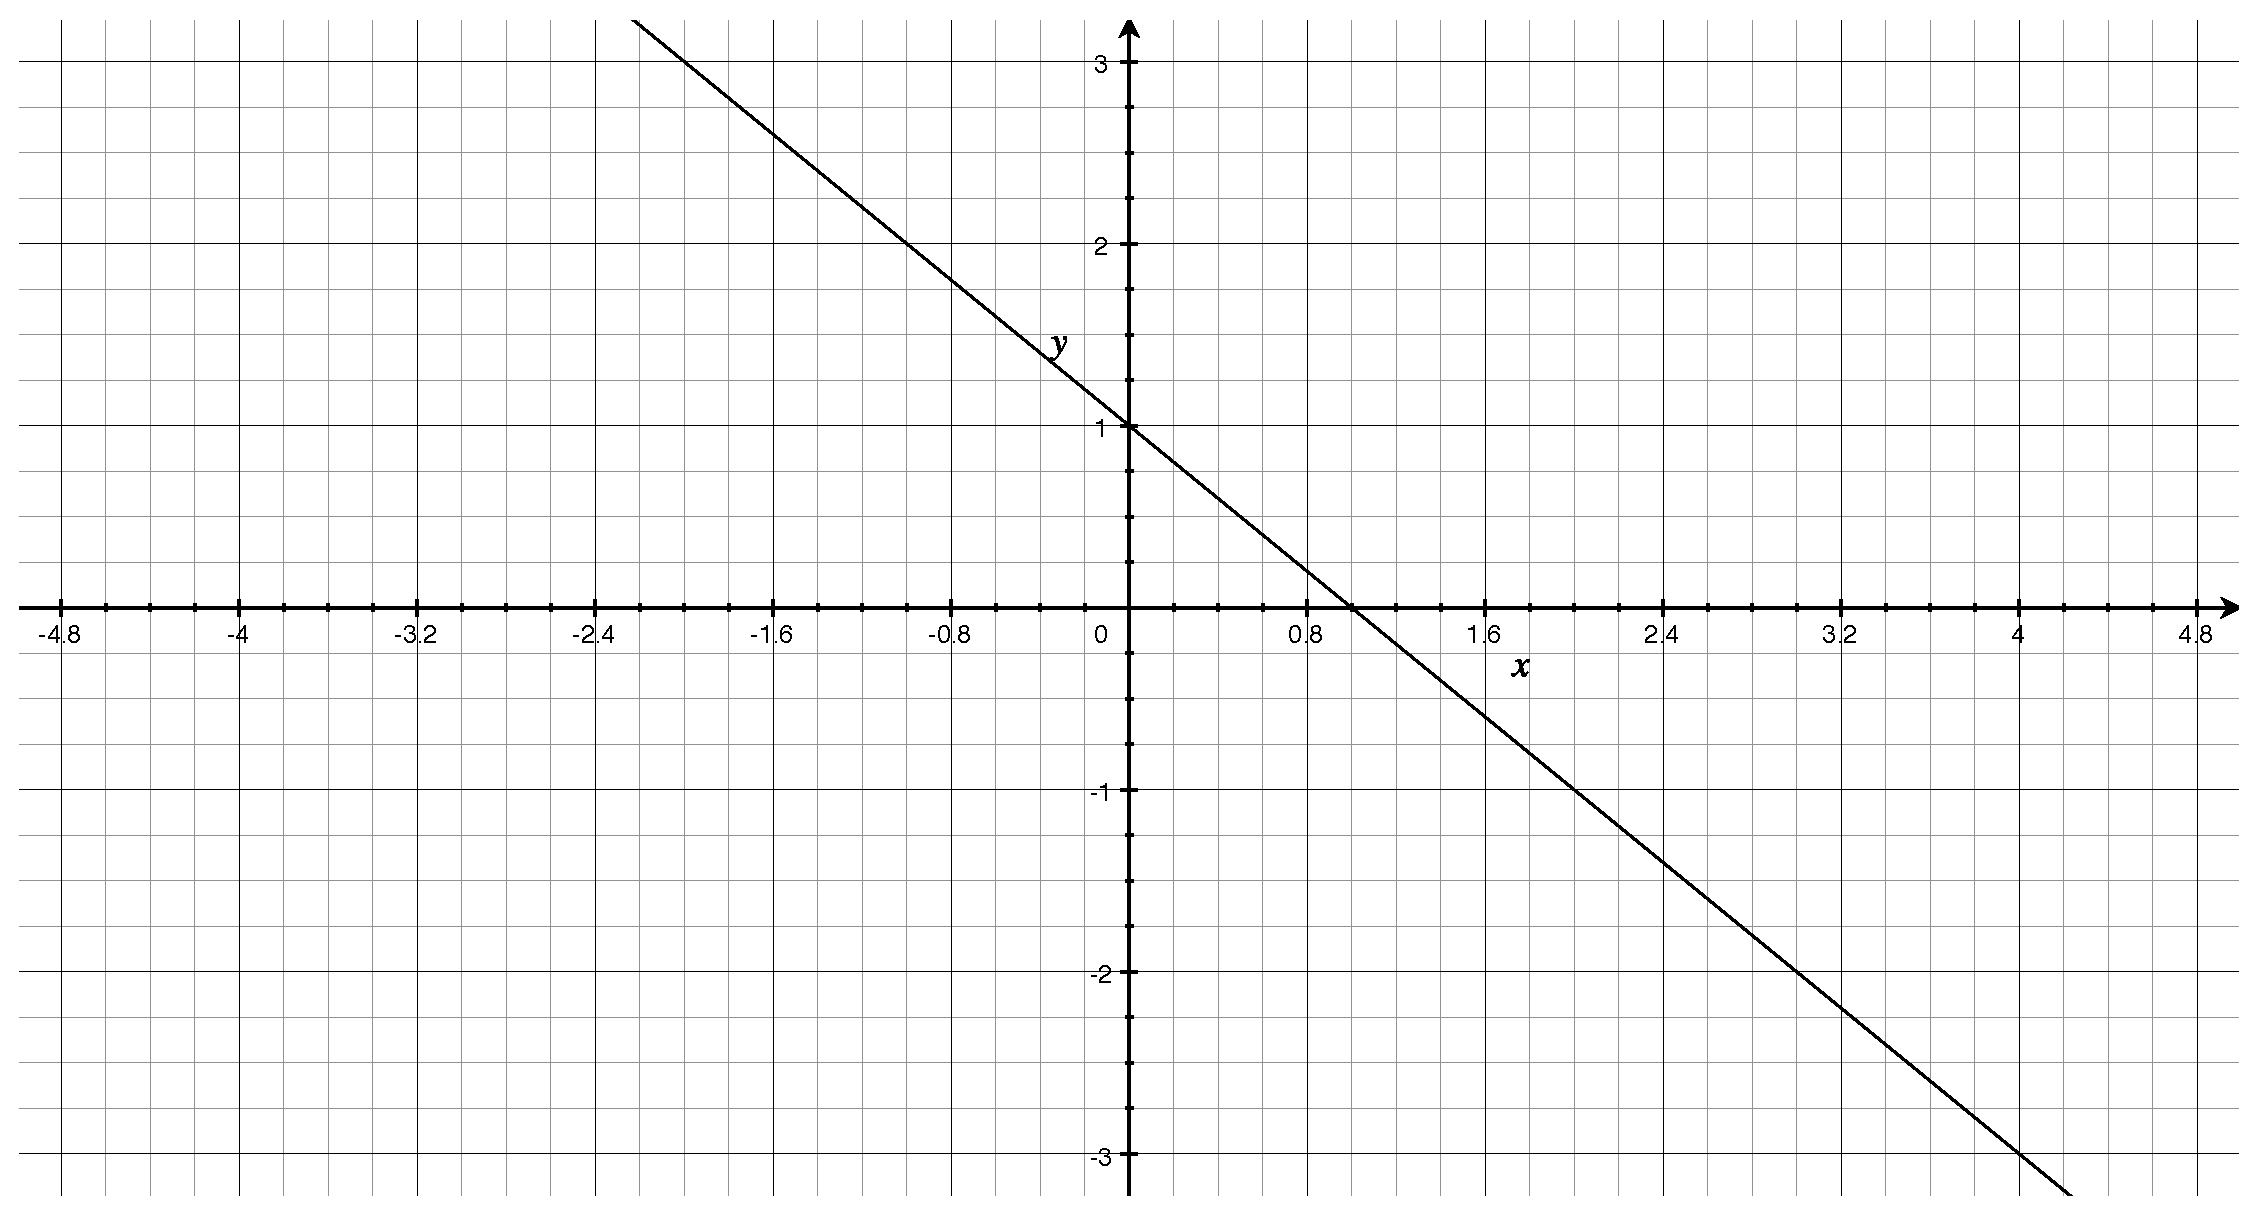
\includegraphics[scale=0.8]{problem7.eps}
%   \caption*{Problem 7}
% \end{figure}

% \begin{tabular}{cc}
%   \toprule
%   period & amplitude \\
%   \midrule
%   value one & value two
%   \bottomrule
% \end{tabular}

\printanswers

\ifprintanswers 
  \usepackage{2in1, lscape} 
\fi

\date{June 26, 2013}
\author{}
\title{Math 141 \\ Homework 16}

\begin{document}

  \maketitle

  \section{Homework}

  Section 4.4: 

  \ifprintanswers
    \pagebreak
  \fi

  \section{Extra Credit}
  Section 4.4: TO DO

  \ifprintanswers
    \begin{description}
      \item[61]
        \begin{align*}
          - \log(x - \sqrt{x^2 - 1}) &= \log(x - \sqrt{x^2 - 1})^{-1} \\
                                     &= \log \frac{1}{x - \sqrt{x^2 - 1}} \\
                                     &= \log \left[ \frac{1}{x - \sqrt{x^2 - 1}} \cdot \frac{x + \sqrt{x^2 - 1}}{x + \sqrt{x^2 - 1}} \right] \\
                                     &= \log \left[ \frac{x + \sqrt{x^2 - 1}}{x^2 - (x^2 - 1)} \right] \\
                                     &= \log ( x + \sqrt{x^2 - 1} ) \\
        \end{align*}

    \end{description}
  \fi

  \ifprintanswers
    \pagebreak
  \fi

  \section{Review}

  Graph each function
  \begin{enumerate}

    \item $f(x) = x + |x|$ 
      \ifprintanswers
        TO DO
      \fi

  \end{enumerate}

  \ifprintanswers
    \section{Section 4.4}

    \begin{description}

      \item[1] 
        \begin{align*}
          \log_3 \sqrt{27} &= \log_3 27^{1/2} \\
                           &= \frac{1}{2} \log_3 27 \\
                           &= \boxed{\frac{3}{2}} \\
        \end{align*}

    \end{description}

  \else
    \vspace{5 cm}
    \begin{quote}
      \begin{em}
        TO DO
      \end{em}
    \end{quote}

    \hspace{1 cm} --Peter Kropotkin
  \fi

\end{document}

